%%%%%%%%%%%%%%%%%%%%%%%%%%%%%%%%%%%%%%%%%%%%%%%%%%%%%%%%%%%%%%%%%%%%%%%%%%%%%%%%
%% Title (en): Multiagent Systems and Organizations                           %%
%% Title (cs): Multiagentní systémy a organizace                              %%
%%                                                                            %%
%% Author: Bc. Lukáš Kúdela                                                   %%
%% Supervisor: Prof. RNDr. Petr Štěpánek, DrSc.                               %%
%%                                                                            %%
%% Academic year: 2011/2012                                                   %%
%%%%%%%%%%%%%%%%%%%%%%%%%%%%%%%%%%%%%%%%%%%%%%%%%%%%%%%%%%%%%%%%%%%%%%%%%%%%%%%%

%%%%%%%%%%%%%%%%%%%%%%%%%%%%%%%%%%%%%%%%%%%%%%%%%%%%%%%%%%%%%%%%%%%%%%%%%%%%%%%%
\section{Example 1: Function Invocations}
%%%%%%%%%%%%%%%%%%%%%%%%%%%%%%%%%%%%%%%%%%%%%%%%%%%%%%%%%%%%%%%%%%%%%%%%%%%%%%%%

% Function invocation organization
This example demonstrates a simple organization - the function invocation.
% Function invocation organization - purpose
The purpose of this organization is to facilitate remote function invocation by grouping two agents: one agent invokes a function and the other one executes it.
% Assumptions
In this example, an agent invokes the factorial function, but it should be obvious that any (computable) function could be invoked this way.

%%%%%%%%%%%%%%%%%%%%%%%%%%%%%%%%%%%%%%%%%%%%%%%%%%%%%%%%%%%%%%%%%%%%%%%%%%%%%%%%
\subsection*{Specification}

%%%%%%%%%%%%%%%%%%%%%%%%%%%%%%%%%%%%%%%%%%%%%%%%%%%%%%%%%%%%%%%%%%%%%%%%%%%%%%%%
\subsubsection*{Organization Part}

% 'Function invocation' organization type
The \textit{Invoke function} organization type (modelled by the \texttt{FunctionInvocation\_Organization} agent class) contains two roles - \textit{Asker} and \textit{Answerer} - and one protocol - \textit{Invoke function}.
% 'function-invocation' organization
\textit{Invoke function} has one instance in the running MAS - the \textit{invoke-function} organization (modelled by the \texttt{invokeFunction\_Organization} agent instance).

% 'Invoker' role
The \textit{Invoker} role (modelled by the \texttt{Invoker\_Role} class) can invoke (not compute) a function to be executed.
% 'Invoker' role - multiplicity, competences & responsibilities
The \textit{Invoker} role is a \textit{single} role.
It has one competence - \textit{Invoke function} - and no responsibilities.

% 'Invoke function' competence
The \textit{Invoke function} competence (modelled by the \texttt{InvokeFunction\_Competence} class) is a competence to invoke a function.
% 'Invoke function' competence - argument & result
It has one argument - the function argument - and one result - the function value. 

% 'Executer' role
The \textit{Executer} role (modelled by the \texttt{Executer\_Role} class) can execute a function upon its invocation.
% 'Execute' role - multiplicity, competences & responsibilities
The \textit{Executer} role is a \textit{single} role.
It has no competences and one responsibility - \textit{Execute function}.

% 'Execute function' responsibility
The \textit{Execute function} responsibility (modelled by the \texttt{ExecuteFunction\_Responsibility} class) is a responsibility to execute a function together for some argument.
% 'Execute function' responsibility - argument & result
It has one argument - the function argument - and one result - the function value.

%%%%%%%%%%%%%%%%%%%%%%%%%%%%%%%%%%%%%%%%%%%%%%%%%%%%%%%%%%%%%%%%%%%%%%%%%%%%%%%%
\subsubsection*{Protocol Part}

% 'Invoke function' protocol
The \textit{Invoke function} protocol (modelled by the \texttt{InvokeFunctionProtocol} class) is a protocol through (ALT: via) which an \textit{Invoker} (the initiator party, modelled by the \texttt{InvokeFunction\_InitiatorParty}) requests an \textit{Executor} (the responder party, modelled by the \texttt{InvokeFunction\_RespodnerParty}) to execute a function (the factorial function in this example).

% 'Invoke function request' message
The \textit{Invoke function request} message (modelled by the \texttt{InvokeFunctionRequestMessage} class) is a message sent by an \textit{Invoker} to an \textit{Executor} requesting the latter to execute a function for a particular argument.

% 'Invoke function reply' message
The \textit{Invoke function reply} message (modelled by the \texttt{InvokeFunctionReplyMessage} class) is a message sent by an \textit{Executer} to an \textit{Invoker} informing the latter about the value of the executed function.

\subsubsection*{Player Part}

% 'Uncapabler' player type
The \textit{Uncapabler} player type (modelled by the \texttt{Uncapabler\_Player} agent class) is a player with no capabilities.
It has one instance in the running MAS - \textit{player1}.
% 'player1' player
\textit{player1} (modelled by the \texttt{player1} agent instance) intends to enact the \textit{Invoker} role in the \textit{invoke-function} organization and to perform the role's \textit{Invoke function} competence - to invoke a function to be executed by the player of the \textit{Executer} role.

% 'Factorial computer' player type
The \textit{Factorial computer} player type (modelled by the \texttt{FactorialComputer\_Player} agent class) is a player capable of computing (ALT: evaluating) the factorial function.
It has one instance in the running MAS - \textit{player2}.
% 'player2' player
The intention of \textit{player2} (modelled by the \texttt{player2} agent instance) is to enact the \textit{Executer} role in the \textit{invoke-organization} organization and perform the role's \textit{Execute function} responsibility - to execute the function invoked by the player of the \textit{Invoker} role.

%%%%%%%%%%%%%%%%%%%%%%%%%%%%%%%%%%%%%%%%%%%%%%%%%%%%%%%%%%%%%%%%%%%%%%%%%%%%%%%%
\subsection*{Manifestation}

%%%%%%%%%%%%%%%%%%%%%%%%%%%%%%%%%%%%%%%%%%%%%%%%%%%%%%%%%%%%%%%%%%%%%%%%%%%%%%%%
\subsubsection*{Stage 1: Role Enactment}

% Figure: Stage 1: Role enactment
\begin{figure}[H]
	\centering
	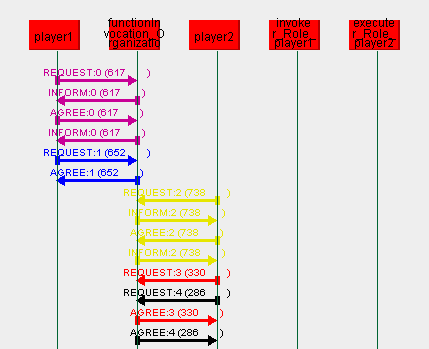
\includegraphics[width=\textwidth]{images/example1-stage1.png}
	\caption{Stage 1: Role enactment}
	\label{figure:example1-stage1}
\end{figure}

% Purple
The \textbf{purple} interaction scenario between \textit{player1} and the \textit{function-invocation} organization follows the \textit{Enact role} protocol.
\textit{player1} requests \textit{invoke-function} to enact the \textit{Invoker} role (1\textsuperscript{st} message) and is informed about the role's responsibilities (2\textsuperscript{nd} message) .
Since \textit{Invoker} has no responsibilities, \textit{player1} agrees that it can indeed enact the role (3\textsuperscript{rd} message).
\textit{invoke-organization} then creates the \textit{invoker-player1} position (modelled by the \texttt{invoker\_Role\_player1} agent instance) and informs \textit{player1} of its AID (4\textsuperscript{th} message).

% Blue
The \textbf{blue} interaction scenario between \textit{player1} and the \textit{function-invocation} organization follows the \textit{Subscribe to event} protocol.
\textit{player1} requests \textit{invoke-function} to subscribe to the \textit{Role activated} event (1\textsuperscript{st} message) and \textit{function-invocation} agrees (2\textsuperscript{nd} message).

% Yellow
The \textbf{yellow} interaction scenario between \textit{player2} and the \textit{invoke-function} organization follows the \textit{Enact role} protocol.
\textit{player2} requests \textit{invoke-function} to enact the \textit{Executer} role (1\textsuperscript{st}) and is informed about the role's responsibilities (2\textsuperscript{nd} message).
Since \textit{player2} can perform one \textit{Executer}'s responsibility - the \textit{Execute function} responsibility - it agrees that it can indeed enact the role (3\textsuperscript{rd} message).
\textit{invoke-function} then creates the \textit{executer-player2} position (modelled by the \texttt{executer\_Role\_player2} agent instance) and informs \textit{player2} of its AID (4\textsuperscript{th} message).

% Red
The \textbf{red} interaction scenario between t\textit{player2} and the \textit{function-invocation} organization follows the \textit{Subscribe to event} protocol.
\textit{player2} requests \textit{invoke-function} to subscribe to the \textit{Role activated} event (1\textsuperscript{st} message) and \textit{function-invocation} agrees (2\textsuperscript{nd} message).

% Black
The \textbf{black} interaction scenario between \textit{player2} and the \textit{function-invocation} organization follows the \textit{Subscribe to event} protocol.
\textit{player2} requests \textit{invoke-function} to subscribe to the \textit{Role deactivated} event (1\textsuperscript{st} message) and \textit{function-invocation} agrees (2\textsuperscript{nd} message).

%%%%%%%%%%%%%%%%%%%%%%%%%%%%%%%%%%%%%%%%%%%%%%%%%%%%%%%%%%%%%%%%%%%%%%%%%%%%%%%%
\subsubsection*{Stage 2: Role Activation}

% Figure: Stage 2: Role activation
\begin{figure}[H]
	\centering
	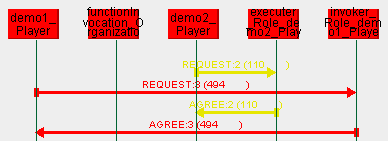
\includegraphics[width=\textwidth]{images/example1-stage2.png}
	\caption{Stage 2: Role activation}
	\label{figure:example1-stage2}
\end{figure}

% Magenta
The \textbf{magenta} interaction scenario between \textit{player1} and the \textit{invoker-player1} position follows the \textit{Activate role} protocol.
\textit{player1} requests \textit{invoker-player1} to activate the role (1\textsuperscript{st} message) and the position promptly agrees (2\textsuperscript{nd} message).

% Cyan
The \textbf{cyan} interaction scenario between the \textit{invoke-function} organization and \textit{player2} follows the \textit{Publish event} protocol.
\textit{invoke-organization} raises a \textit{Role activated} event (for the \textit{Invoker} role) and \textit{player2} handles it by activating its \textit{Executer} role (the \textbf{pink} interaction scenario).

% Pink
The \textbf{pink} interaction scenario between \textit{player2} and the \textit{executer-player2} position follows the \textit{Activate role} protocol.
\textit{player2} requests \textit{executer-player2} to activate the role (1\textsuperscript{st} message) and the position immediately agrees (2\textsuperscript{nd} message).

% Dark green
The \textbf{dark green} interaction scenario between the \textit{invoke-function} organization and \textit{player1} follows the \textit{Publish event} protocol.
\textit{invoke-organization} raises a \textit{Role activated} event (for the \textit{Executer} role) and \textit{player1} handles it by invoking the \textit{Invoke function} competence (the \textbf{light green} interaction scenario).

%%%%%%%%%%%%%%%%%%%%%%%%%%%%%%%%%%%%%%%%%%%%%%%%%%%%%%%%%%%%%%%%%%%%%%%%%%%%%%%%
\subsubsection*{Stage 3: Competence and Responsibility Invocation}

% Figure: Stage 3: Competence and responsibility invocation
\begin{figure}[H]
	\centering
	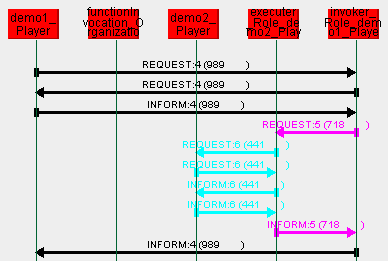
\includegraphics[width=\textwidth]{images/example1-stage3.png}
	\caption{Stage 3: Competence and responsibility invocation}
	\label{figure:example1-stage3}
\end{figure}

% Note - `Invoke competence' protocol vs. 'Invoke function' competence
In the following discussion, is is important to keep in mind that the \textit{Invoke competence} protocol is being used to invoke the \textit{Invoke function} competence.
Understanding the distinction between these two usages of the word `invoke' is a prerequisite to understanding the discussion of Stage 3.

% Light green
The \textbf{light green} interaction scenario between \textit{player1} and the \textit{invoker-player1} position follows the \textit{Invoke competence} protocol.
\textit{player1} requests \textit{invoker-player1} to invoke the \textit{Invoke function} competence (1\textsuperscript{st} message) and is in turn requested to provide the competence argument (2\textsuperscript{nd} message).
\textit{player1} then promptly informs \textit{invoker-player1} about the argument (3\textsuperscript{rd} message).
After \textit{invoker-player1} executes the competence (the \textbf{purple} interaction scenario), it informs \textit{player1} about its result (4\textsuperscript{th} message).

% Purple
The \textbf{purple} interaction scenario between the \textit{initiator-player1} and \textit{executer-player2} positions follows the \textit{Invoke function} protocol.
\textit{initiator-player1} requests \textit{executer-player2} to execute a particular function (factorial) for a particular argument (10, 1\textsuperscript{st} message).
\textit{executer-player2}, after invoking the \textit{Execute function} responsibility on its player (the \textbf{blue} interaction scenario), informs \textit{invoker-player1} about the function return value (3628800, 2\textsuperscript{nd} message).

% Blue
The \textbf{blue} interaction scenario between the \textit{executer-player2} position \textit{player2} follows the \textit{Invoke responsibility} protocol.
\textit{executer-player2} requests \textit{player2} to invoke the \textit{Execute function} responsibility (1\textsuperscript{st} message) and is in turn requested to provide the responsibility argument (2\textsuperscript{nd} message).
\textit{executer-player2} then immediately informs \textit{player2} about the argument (3\textsuperscript{rd} message).
After \textit{player2} executes the responsibility, it informs \textit{executer-player2} about its result (4\textsuperscript{th} message).

%%%%%%%%%%%%%%%%%%%%%%%%%%%%%%%%%%%%%%%%%%%%%%%%%%%%%%%%%%%%%%%%%%%%%%%%%%%%%%%%
\subsubsection*{Stage 4: Role Deactivation}

% Figure: Stage 4: Role deactivation
\begin{figure}[H]
	\centering
	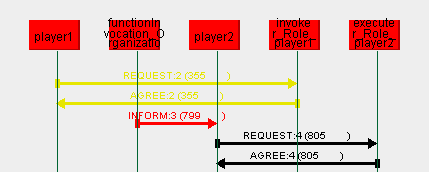
\includegraphics[width=\textwidth]{images/example1-stage4.png}
	\caption{Stage 4: Role deactivation}
	\label{figure:example1-stage4}
\end{figure}

% Yellow
The \textbf{yellow} interaction scenario between \textit{player1}  and the \textit{invoker-player1} position.
\textit{player1} requests \textit{invoker-player1} to deactivate the role (1\textsuperscript{st} message) and the position promptly agrees (2\textsuperscript{nd} message).

% Red
The \textbf{red} interaction scenario between the \textit{invoke-function} organization and \textit{player2} follows the \textit{Publish event} protocol.
\textit{invoke-organization} raises a \textit{Role deactivated} event (for the \textit{Invoker} role) and \textit{player2} handles it by deactivating its \textit{Executer} role (the \textbf{light green} interaction scenario).

% Black
The \textbf{black} interaction scenario between \textit{player2} and the \textit{executer-player2} position.
\textit{player2} requests \textit{executer-player2} to deactivate the role (1\textsuperscript{st} message) and the position immediately agrees (2\textsuperscript{nd} message).

%%%%%%%%%%%%%%%%%%%%%%%%%%%%%%%%%%%%%%%%%%%%%%%%%%%%%%%%%%%%%%%%%%%%%%%%%%%%%%%%
\subsubsection*{Stage 5: Role Deactment}

% Figure: Stage 5: Role deactment
\begin{figure}[H]
	\centering
	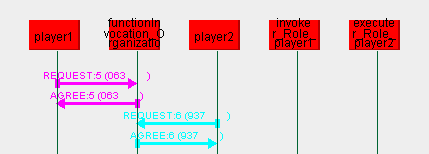
\includegraphics[width=\textwidth]{images/example1-stage5.png}
	\caption{Stage 5: Role deactment}
	\label{figure:example1-stage5}
\end{figure} 

% Magenta
The \textbf{magenta} interaction scenario between \textit{player1} and the \textit{invoke-function} organization.
\textit{player1} requests \textit{invoke-function} to deact the \textit{Invoker} role (1\textsuperscript{st} message) and the organization promptly agrees (2\textsuperscript{nd} message).

% Cyan
The \textbf{cyan} interaction scenario between \textit{player2} and the \textit{invoke-function} organizations.
\textit{player2} requests \textit{invoke-function} to deact the \textit{Executer} role (1\textsuperscript{st} message) and the organization immediately agrees (2\textsuperscript{nd} message).